\chapter{Hauptteil}

\section{Technische Architektur}

\begin{figure}[htb]
    \centering
    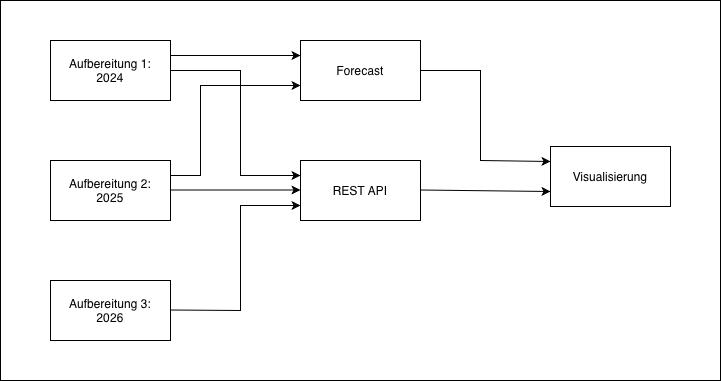
\includegraphics[width=\textwidth]{Abbildungen/Containerarchitektur.png}
    \caption[Containerarchitektur]{Containerarchitektur\footnotemark}
    \label{fig:containerarchitektur}
\end{figure}
\footnotetext{Eigene Darstellung.}

Die realisierte Systemarchitektur setzt sich aus sechs funktional getrennten Docker-Containern zusammen, die über ein gemeinsames Bridge-Netzwerk miteinander kommunizieren (vgl. Abbildung \ref{fig:containerarchitektur}). Das Fundament bilden drei identische Instanzen des Aufbereitungsdienstes (\texttt{aa\_aufbereitung\_1} bis \texttt{aa\_aufbereitung\_3}), die durch containerindividuelle Volume-Mounts jeweils spezifische Datenzeiträume verarbeiten: die Perioden 2025 sowie Januar 2026. Die mehrfache Instanziierung desselben Container-Images demonstriert das Kernprinzip horizontaler Skalierbarkeit – eine einmal definierte Laufzeitumgebung kann ohne Anpassung des Anwendungscodes für unterschiedliche Eingabedaten repliziert werden (vgl. Merkel 2014, S.~4~f.). Jede Instanz exponiert eine REST-konforma HTTP-Schnittstelle auf Port 8080 und stellt aufbereitete Datensätze sowie Spalteninformationen für nachgelagerte Dienste bereit. Um eine kontrollierte Startreihenfolge zu gewährleisten, definiert \texttt{docker-compose.yaml} Gesundheitsprüfungen auf Basis von HTTP-Anfragen sowie \texttt{depends\_on}-Bedingungen, die sicherstellen, dass kein nachgelagerter Dienst startet, bevor alle Aufbereitungsinstanzen betriebsbereit sind (vgl. Stoneman 2020, S.~14~ff.).

Der Forecast-Container (\texttt{aa\_forecast}) bezieht die aufbereiteten Rohdaten über konfigurierbare HTTP-Verbindungen aus allen drei Aufbereitungsinstanzen, führt sie zu einem gemeinsamen DataFrame zusammen und stellt darauf basierend statistische Vorhersagemodelle über eine eigene REST-API auf Port 9000 bereit. Der API-Container (\texttt{aa\_api}) hingegen aggregiert die historischen Daten ausschließlich nach zeitlichen Dimensionen und dient als stabiler Datenzugangspunkt für die Visualisierungsschicht. Den Abschluss des Datenflusses bildet der Visualisierungs-Container (\texttt{aa\_visual}), der eine interaktive Webanwendung auf Basis von Streamlit bereitstellt und sowohl historische als auch prognostizierte Kennzahlen grafisch aufbereitet. Die konsequente Diensttrennung entspricht dem Microservice-Paradigma, das funktionale Einheiten in lose gekoppelte, unabhängig deploybare Dienste zerlegt und so eine gezielte Skalierung einzelner Komponenten ohne Beeinträchtigung des Gesamtsystems ermöglicht (vgl. Newman 2015, S.~1~ff.).

\section{Aufbereitung der Daten}

Die Datenaufbereitung gliedert sich in drei aufeinanderfolgende Phasen: den Datenimport, die Bereinigung sowie die Merkmalsgenerierung. Der Import unterstützt sowohl das CSV- als auch das spaltenorientierte Apache-Parquet-Format, wobei Parquet-Dateien blockweise über PyArrow eingelesen werden, um den Hauptspeicherverbrauch zu kontrollieren (vgl. Vohra 2016, S.~11~f.). CSV-Dateien werden mittels \texttt{pandas} in Chunks von 100.000~Zeilen verarbeitet; im Testbetrieb wird über zufälliges Zeilen-Sampling der Datensatz auf einen repräsentativen Bruchteil reduziert, um Entwicklungszyklen zu beschleunigen. Sämtliche Zeitstempelfelder (\texttt{tpep\_pickup\_datetime}, \texttt{tpep\_dropoff\_datetime}) werden in ein einheitliches Zeichenkettenformat überführt, aus dem Jahr, Monat, Tag und Stunde als separate numerische Spalten extrahiert werden (vgl. McKinney 2017, S.~97~ff.).

Die Bereinigungsroutine entfernt systematisch unplausible Datensätze: Fahrten mit einem Fahrpreis von null oder negativen Werten werden ausgeschlossen, ebenso Fahrtstrecken außerhalb des Intervalls $(0, 100]$~Meilen sowie Passagierzahlen kleiner eins oder größer sechs. Extremwerte des Fahrpreises oberhalb des 99,5.~Perzentils werden gekappt, um den Einfluss vereinzelter Datenerfassungsfehler auf nachgelagerte Modelle zu begrenzen.

Die Merkmalsgenerierung überführt die Rohdaten in ein für statistische Modellierung geeignetes Format. Aus dem Abholzeitpunkt werden Wochentag, Wochenendindikator, Jahreszeit sowie binäre Variablen für Feiertage (auf Basis der US-amerikanischen gesetzlichen Feiertage), den Tag vor und nach einem Feiertag sowie die Rush-Hour-Perioden (7–9~Uhr und 16–18~Uhr) abgeleitet. Zur Abbildung der inhärenten Zyklizität zeitlicher Dimensionen werden Wochentag und Monat mittels trigonometrischer Transformation in Sinus- und Kosinuskomponenten überführt:

\begin{equation}
    x_{\sin} = \sin\!\left(\frac{2\pi \cdot t}{T}\right), \quad x_{\cos} = \cos\!\left(\frac{2\pi \cdot t}{T}\right)
\end{equation}

Dabei bezeichnet $t$ den diskreten Zeitindex (Wochentag $0$–$6$ bzw. Monat $1$–$12$) und $T$ die Periodenlänge. Diese Kodierung stellt sicher, dass die Distanz zwischen Montag und Sonntag im Merkmalsraum der intuitiven zyklischen Nähe entspricht – eine Eigenschaft, die lineare Merkmale nicht abbilden können (vgl. Fahrmeir/Tutz 2001, S.~10~f.).

Für Fahrten mit Barzahlung (\texttt{payment\_type}~=~2) weist der Datensatz strukturell fehlende Trinkgeldwerte auf, da Trinkgelder bei dieser Zahlungsart nicht elektronisch erfasst werden. Zur Imputation wird das MICE-Verfahren (\textit{Multiple Imputation by Chained Equations}) eingesetzt, das für jede unvollständige Variable ein separates Regressionsmodell spezifiziert und diese Kette konditionaler Modelle iterativ bis zur Konvergenz durchläuft (vgl. van Buuren/Groothuis-Oudshoorn 2011, S.~7~ff.). Die Scikit-learn-Implementierung \texttt{IterativeImputer} verwendet als Prädiktoren Gesamtbetrag, Fahrpreis und Fahrtdistanz; negative Imputationswerte werden anschließend auf null begrenzt, da Trinkgelder definitionsgemäß nicht negativ sein können (vgl. Pedregosa et~al. 2011, S.~2826). Durch dieses Vorgehen wird auf den listenweisen Ausschluss von Barzahlungsfahrten verzichtet, was die Stichprobengröße erhält und potenzielle Verzerrungen durch systematisch fehlende Werte reduziert (vgl. Little/Rubin 2002, S.~41~ff.).

Die aufbereiteten Daten werden als vollständiger JSON-kodierter DataFrame über den \texttt{/miced\_data}-Endpunkt der jeweiligen Aufbereitungsinstanz bereitgestellt; die Spaltenliste ist separat über \texttt{/columns} abrufbar und wird beim Start nachgelagerter Dienste zur Kompatibilitätsprüfung herangezogen.

\section{Modellierung und Prognose}

Der Forecast-Dienst realisiert eine anfrage-gesteuerte statistische Modellierung: Für jede eingehende HTTP-Anfrage werden Aggregationsmethode, Gruppierungsdimensionen und Zielvariable aus den URL-Parametern extrahiert, ein Modell auf den entsprechend aggregierten Trainingsdaten angepasst und Vorhersagen für den Zielzeitraum 2026 generiert.

\subsection{Merkmalsauswahl und Aggregation}

Abhängig vom angefragten Zeitgranular werden unterschiedliche Merkmalssätze aktiviert: Für tagesgenaue Anfragen fließen zyklische Wochentag-Kodierungen sowie alle binären Tagesmerkmale (Wochenende, Feiertag, Rush-Hour etc.) in die Modellformel ein; für monatliche Anfragen werden die trigonometrischen Monatskodierungen hinzugefügt. Werden stündliche Dimensionen wie \texttt{pickup\_hour} einbezogen, ergänzt der Dienst automatisch den Rush-Hour-Indikator. Die Zielvariable und alle kategorialen Prädiktoren werden über eine \texttt{patsy}-Formel spezifiziert, wobei kategoriale Variablen automatisch als Dummy-Variablen kodiert werden. Für Vorhersagen wird ein kartesisches Produkt aller zulässigen Merkmalsausprägungen als Prädiktionsrahmen aufgespannt, sodass vollständige Vorhersagegitter entstehen.

\subsection{Modellauswahl und Schätzung}

Je nach Aggregationsmethode der Zielvariablen werden unterschiedliche Modellklassen eingesetzt. Bei Zählaggregationen (\texttt{count}) werden ein Poisson-GLM sowie – zur Behandlung von Überdispersion – ein Negativ-Binomial-GLM angepasst (vgl. Cameron/Trivedi 2013, S.~75~f.). Bei stetigen Zielgrößen (\texttt{mean}) stehen neben dem Gauß-GLM, sofern die Zielvariable strikt positiv ist, zusätzlich ein Gamma- sowie ein Invers-Gauß-GLM zur Verfügung, die asymmetrisch verteilte, rechtsschiefe Größen wie Fahrpreise adäquater modellieren (vgl. McCullagh/Nelder 1989, S.~292~ff.). Ergänzend wird stets ein OLS-Modell (\textit{Ordinary Least Squares}) als Referenzmodell geschätzt. Alle GLM-Parameter werden über Maximum-Likelihood-Schätzung bestimmt (vgl. Nelder/Wedderburn 1972, S.~370~ff.); die Implementierung erfolgt über \texttt{statsmodels} mit patsy-basierter Formelschnittstelle (vgl. Seabold/Perktold 2010, S.~93).

Für stetige Zielgrößen wird vor der Modellanpassung eine logarithmische Transformation der Zielvariablen mittels $\log(1 + y)$ vorgenommen. Diese Varianzstabilisierung begegnet der typischen rechtsschieven Verteilung von Betragsgrößen und verbessert die Anpassungsgüte linearer Prädiktoren; die Rücktransformation der Vorhersagen erfolgt über $\exp(\hat{y}) - 1$ (vgl. Fahrmeir/Tutz 2001, S.~18~f.).

Zur Modellbewertung liefert der Dienst neben den eigentlichen Vorhersagen eine Zusammenfassung aller angepassten Modelle, die Koeffizientenschätzungen, zugehörige $p$-Werte, das Akaike-Informationskriterium (AIC) sowie – für das OLS-Modell – das Bestimmtheitsmaß $R^2$ und dessen adjustierte Variante enthält. Das AIC erlaubt einen modellklassenübergreifenden Vergleich unter Berücksichtigung der Modellkomplexität: Ein niedrigerer AIC-Wert indiziert ein günstigeres Verhältnis zwischen Anpassungsgüte und Parameterzahl (vgl. Fahrmeir/Tutz 2001, S.~86~ff.). Die Modellzusammenfassung wird über die API an die Visualisierungsschicht übermittelt und dort tabellarisch nach AIC sortiert dargestellt, sodass Nutzer das leistungsfähigste Modell für den jeweiligen Anwendungsfall identifizieren können.

\section{Visualisierung}

Die Visualisierungsschicht ist als interaktive Webanwendung in Streamlit realisiert und bindet sowohl den historischen API-Dienst als auch den Forecast-Dienst als konfigurierbare Datenquellen ein (vgl. Tamminga 2022, S.~1~f.). Die Seitenleiste erlaubt die kontextadaptive Auswahl von Zeiträumen, Kennzahlen, Aggregationsmethoden und Gruppierungsdimensionen; verfügbare Zeiträume werden dabei dynamisch aus dem \texttt{/data\_summary}-Endpunkt der verbundenen APIs bezogen, sodass die Oberfläche stets nur tatsächlich vorhandene Daten anbietet.

Für die Ergebnisdarstellung stehen fünf Diagrammtypen zur Verfügung: Liniendiagramme für zeitliche Verläufe, Balkendiagramme für ein- und zweidimensionale Vergleiche, Heatmaps zur Darstellung zweidimensionaler Kreuztabellen, Streudiagramme sowie dreidimensionale Streudiagramme für mehrdimensionale Beziehungen. Alle Diagramme werden mit Plotly Express gerendert und sind interaktiv zoom- und filterbar (vgl. Tamminga 2022, S.~1~f.). Oberhalb jeder Visualisierung werden drei Kennzahlen – Summe, Durchschnitt und Datensatzanzahl – als kompakte Metriken hervorgehoben.

Die Anfragestrategie passt sich automatisch an den ausgewählten Zeitgranular an: Bei tagesgenauen Anfragen wird für jeden selektierten Tag eine separate API-Anfrage gestellt und die Ergebnisse anschließend zusammengeführt; bei monatlichen oder jährlichen Anfragen wird entsprechend auf Monats- bzw. Jahresebene aggregiert. Sind sowohl der historische als auch der Forecast-Dienst aktiv, werden Prognose- und Ist-Daten für identische Zeitperioden kombiniert, wobei Duplikate durch Priorisierung des historischen Dienstes aufgelöst werden. Kategoriale Variablen wie Zahlungsart, Anbieter und Tarifcode werden clientseitig auf lesbare Bezeichnungen abgebildet. Über dynamische Filterpanels können Nutzer die dargestellten Merkmalskombinationen interaktiv einschränken; der vollständige Datensatz ist zudem als CSV-Datei exportierbar.

\section{Mögliche Analysen}

Das realisierte System ermöglicht eine Vielzahl deskriptiver und prädiktiver Analysen. Deskriptiv lassen sich Nachfrageschwankungen über Tagesstunden, Wochentage und Monate verfolgen und mit Feiertagen oder Rush-Hour-Perioden in Beziehung setzen. Die Gruppierung nach Zahlungsart erlaubt Rückschlüsse auf Kundenpräferenzen; eine Kreuzauswertung von Anbieter und Tarifzone gibt Hinweise auf räumliche Nachfragekonzentrationen. Durch Gegenüberstellung der imputierten Trinkgelddaten mit Fahrpreisen und Zahlungsarten lassen sich Einflussfaktoren auf das Trinkgeldverhalten explorieren.

Prädiktiv kann das System Zielgrößen wie Fahrtenanzahl, durchschnittlicher Fahrpreis oder Trinkgeldhöhe für beliebige Kombinationen aus Tageszeit, Wochentag und Saisonmerkmalen im Prognosezeitraum 2026 schätzen. Der modellübergreifende Vergleich über das AIC ermöglicht dabei eine datengetriebene Auswahl des geeignetsten Modells je Anwendungsfall. Die Integration von Prognosedaten und historischen Daten in einer gemeinsamen Visualisierung erlaubt schließlich eine unmittelbare visuelle Validierung der Modellgüte.